\documentclass[letterpaper,10pt]{article}

%\setlength{\parindent}{0in}
%\usepackage{fullpage} 
\usepackage{amsmath}
\usepackage{amssymb}
\usepackage{enumerate}
\usepackage{graphicx}
\usepackage[table]{xcolor}
\usepackage{dcolumn}
\oddsidemargin 0.0in
\textwidth 6.5in
\newcolumntype{.}{D{.}{.}{-1}}
\newcommand*{\myalign}[2]{\multicolumn{1}{#1}{#2}}

%opening
\title{Assignment 2}
\author{Steve Mazza}
\date{January 27, 2012}

\begin{document}
\maketitle

\section*{Part 1}
\begin{enumerate}
\item I opened and studied the Excel spreadsheet ignoring the links.
\item A full factorial design would require $2^{4}\times 3 = 48$ possible combinations.
\item
	\begin{enumerate}
	\item According to the Airplane Chart Means a configuration based on A1, B3, C1, D1 would have the longest mean flight distance.
	\item The airplane A1, B3, C1, D1 was not built and tested during the experiment.
	\item According to the Airplane Chart Variances a configuration based on A2, B2, C2, D3 would have the smallest variance in terms of flight distance.
	\item The airplane A2, B2, C2, D3 was not built and tested during the experiment.
	\end{enumerate}
\item This type of experimental design offers a high predictive value at a significant reduction in terms of time and cost due to the reduced number of tests required to produce accurate results.
\end{enumerate}

\section*{Part 2}
Assuming an $\alpha$ of 0.05, there appears to be a statistically significant difference between the \emph{Concept} and \emph{Operational} data sets but not between the \emph{Concept} and \emph{Prototype} data sets.  

The results are calculated on the attached spreadsheet and summarized below.

\begin{table}[htdp]
\begin{center}
\begin{tabular}{l.}
\hline
\myalign{c}{\textbf{Data Sets}} & \myalign{.}{\textbf{p-value}} \\
\hline
Concept vs. Prototype & 1.0 \\
Concept vs. Operational & 0.00967 \\
Prototype vs. Operational & 0.03058 \\
\hline
\end{tabular}
\end{center}
\end{table}

The \emph{Concept} data is well supported by the \emph{Prototype} data.  The \emph{Operational} data does not support the previous two results well.  Reference the chart below.  \emph{Concept} is labeled 1, \emph{Prototype} is labeled 2, and \emph{Operational} is labeled 3.  The scale on the left is linear and represents the actual data.

\begin{center}
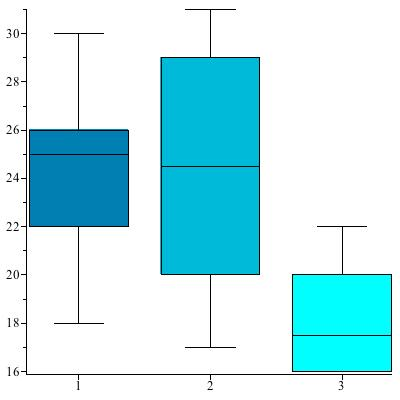
\includegraphics[scale=0.75]{image1.jpg}
\end{center}

Additionally worth notiing, there is almost twice the variance in the \emph{Prototype} (30.26667) as in the \emph{Concept} (16.66667) which means that consistent results will be more difficult to reproduce.  While the \emph{Operational} data has by far the lowest variance (5.76667), it's results are still least correlated to the \emph{Concept}.

\end{document}